\section{Using ML for the Keyspace}
\label{sec:ml-for-the-keyspace}

We proved in the previous section that an optimial policy, based on the read
burstiness at the beginning of the run,  exists for a 100K growth rate on 8
nodes, but we cannot re-do this analysis for every workload, system, and
parameter permutation.  Fortunately,
Section~\S\ref{sec:parsplice-keyspace-analysis} shows that the keyspace size
and activity is structured. so rather than finding policies by hand again for
every cluster size, growth rate, and temperature, in this section we use
machine learning to inform the Mantle policy engine.  Machine learning is good
at two things: handling large design spaces and matching patterns. Our keyspace
analysis in Section~\ref{sec:parsplice-keyspace-analysis} demonstrated a large
design space and Figure~\ref{fig:motivation-regimes} shows 4 workload regimes:
one plateau of redundant reads at the beginning, decreasing requests per
second, and then two plateaus of steady requests per second. We start with a
simple clustering algorithm to attack this multi-dimensional design space
problem and detect workload regimes.

% implementation: 
We feed the read request rate from the 100K and 1M runs in
Figure~\ref{fig:motivation-regimes} into the K-means clustering algorithm as
(timestamp, ops/second) tuples\footnote{Note that the magnitudes are different
because Figure~\ref{fig:motivation-regimes} was run with keyspace tracing on,
which reduces performance}. We weight the timestamp and ops/second equally and
set the number of clusters to be 4.  We chose this initial K  based on visual
inspection of Figure~\ref{fig:motivation-regimes} Knowing that the setup
parameters transform the request rates temporally or spatially, this same
initial K should work for all setups. Once the algorithm identifies the
workload regimes, we select the start of the third regime as the point to
switch to a fixed sized cache because the request rate has lowered to
sustainable levels for the persistent database.

We plot throughput over time in Figure~\ref{fig:futurework-regimes} and
color each point with its assigned group. The black stars are the centroids,
also known as the center of K-means groups.  We run the algorithm for a variety
of request rate traces but only show the setups from
Figure~\ref{fig:motivation-regimes}. We also annotate the graphs with the
suggested cache size, which is calculated by looking up the timestamp for the
third regime that corresponds to the keyspace size in our performance counters.

% results: 1. ideentifies 4 phases, 2. picks different timestamps for the third
% regime, suggests proper key values.
The algorithm properly identifies the 4 workload phases: the plateau of
redundant reads, the phase with a large decrease in request rate, and the two
plateaus of steady read requests. It also picks different timestamps for the
start of the third regime, which aligns with our keyspace analysis and our
assertion that the growth parameters affect how long it takes the workload to
reach a certain phase.  Finally, the algorithm picks reasonable values for the
key cache size. The 100K growth rate selects a 55K cache size, which is between
our benchmarked optimal threshold for the high watermark value chosen to
absorb the read burst (100K) and the lower cache size we limit the system to
after the initial burst (10K). This result both reaffirms the results from the
previous section and provides hope that we can avoid lengthy paramaters sweeps
for ParSplice in the future.

\begin{figure}[t]
\noindent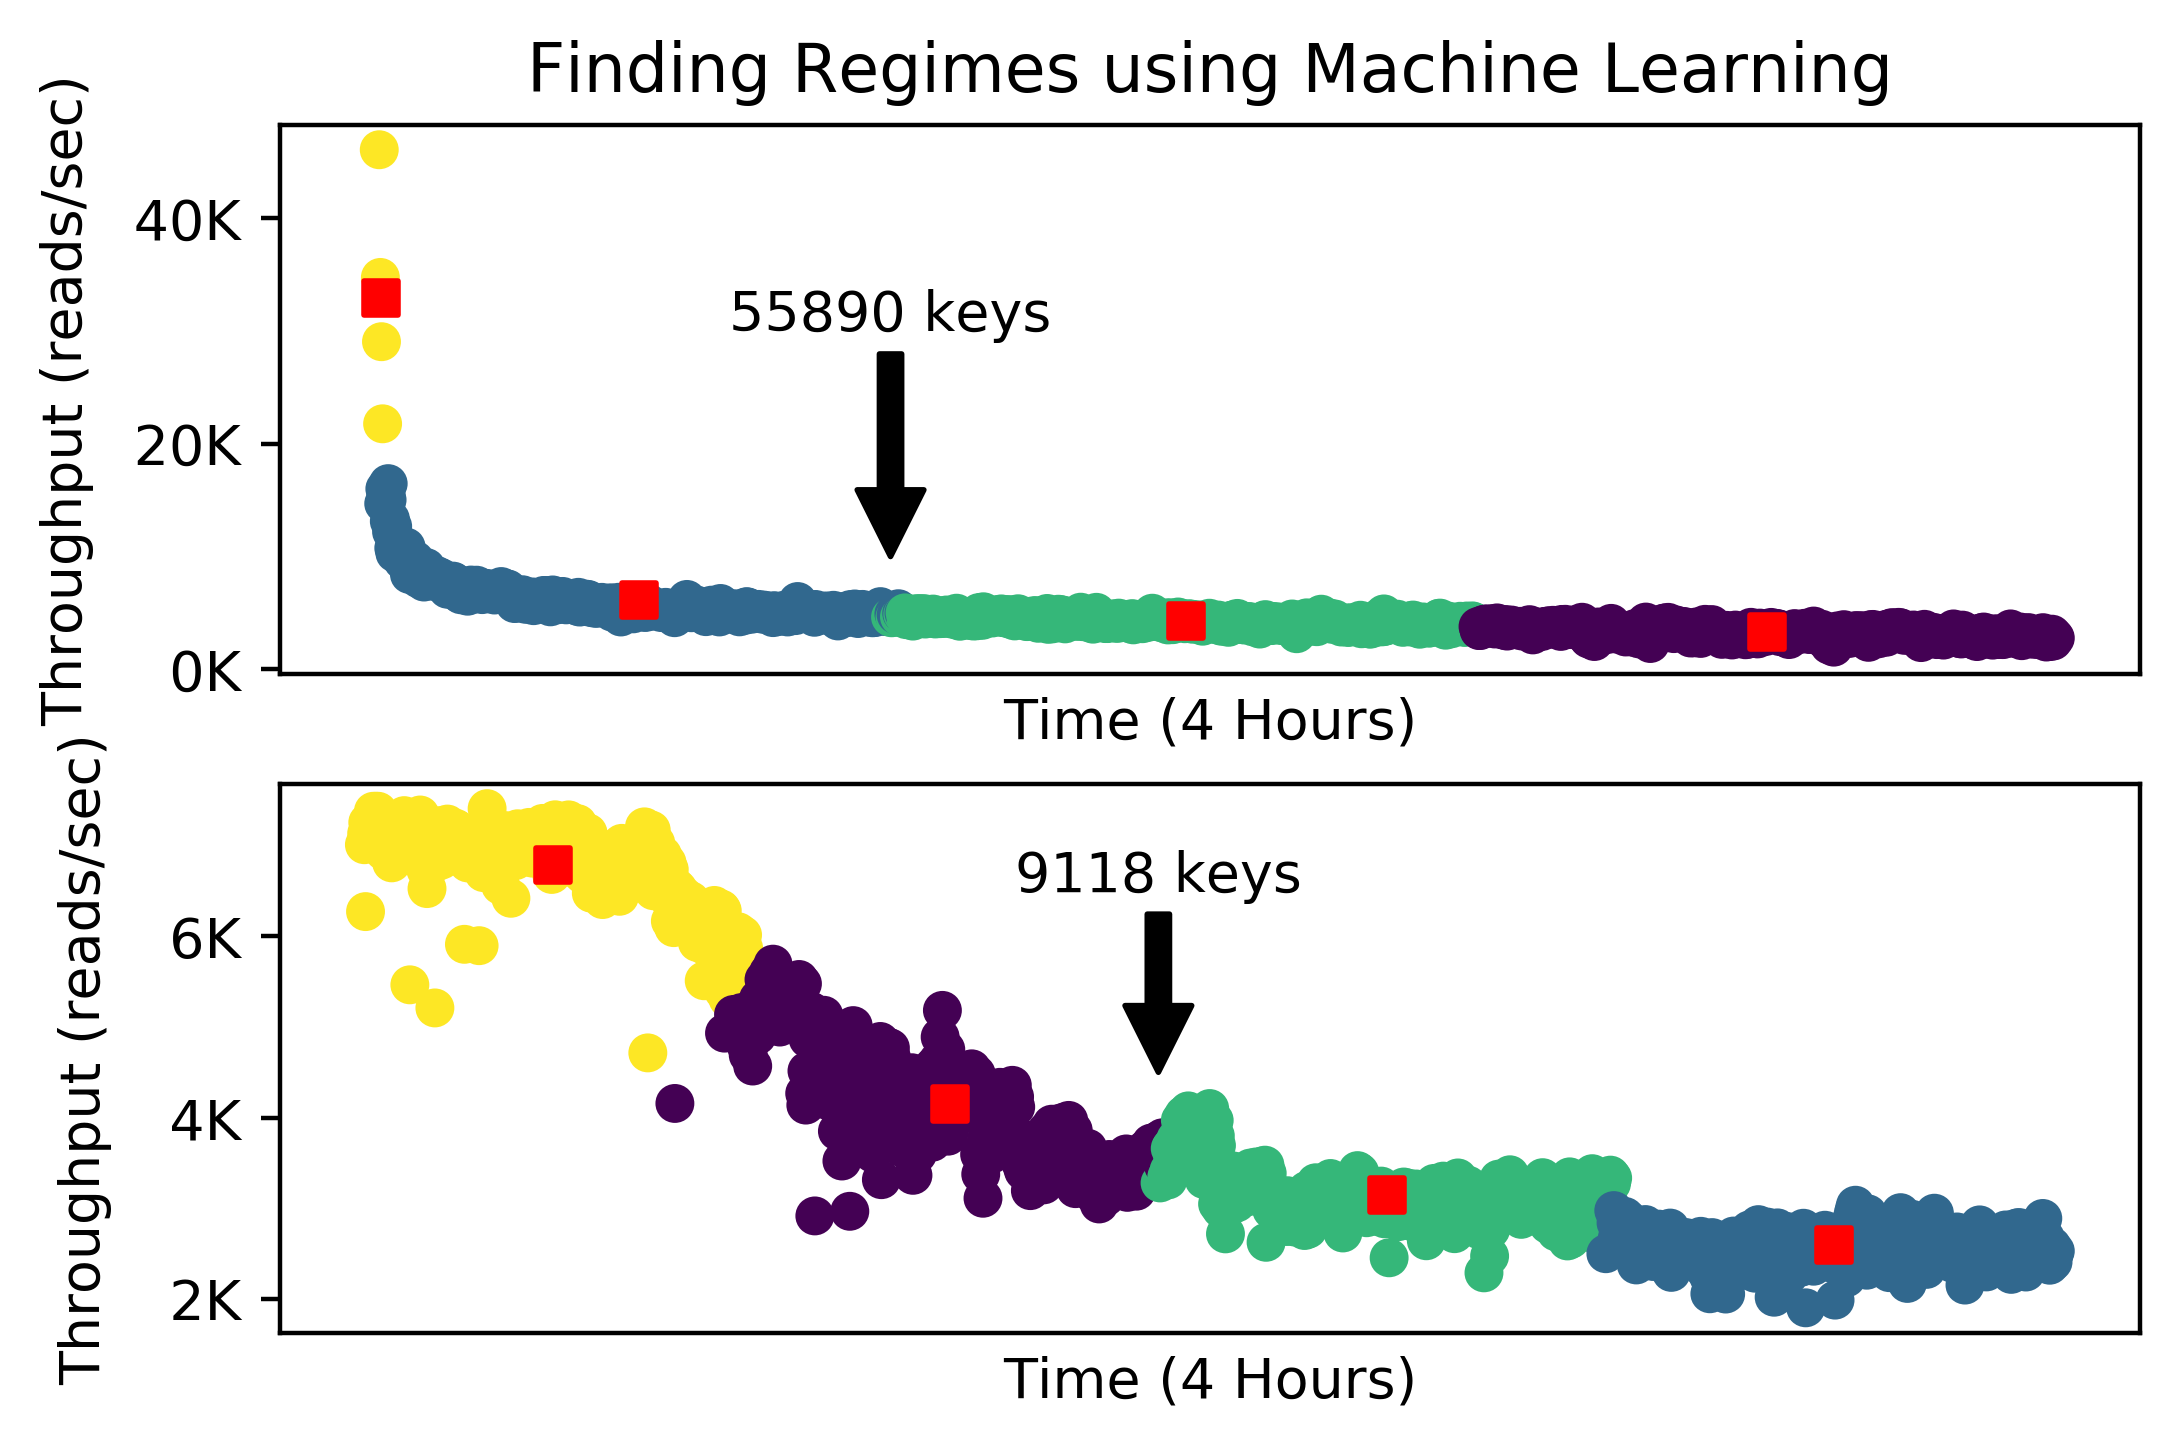
\includegraphics[width=0.4\textwidth]{figures/futurework-regimes.png}\\
  \caption{Learning the workload regimes with K-Means clustering helps pick
  keyspace size thresholds that can be fed into a dynamic load balancing policy
  engine, like Mantle. Specifying 4 clusters and selecting the third for
  informing the policy switch returns keyspace size thresholds similar to the
  values we found by hand in
  Section~\S\ref{sec:the-need-for-dynamic-load-balancing-policies}.
\label{fig:futurework-regimes}}
\end{figure}
